% !TeX root = proyecto.tex
%=========================================================
\chapter{Modelo de la interacción}	
\label{cap:modInteraccion}

\cdtInstrucciones{Introduzca el capítulo indicando su contenido y organización.}	

\cdtInstrucciones{Utilice este capítulo para describir todos los detalles de la interacción con el usuario, describiendo elementos d eusabilidad, ergonomía, psicología,  arqjuitectura de información y repreentación.}

Este capítulo describe ...

\section{Modelo de navegación}

\cdtInstrucciones{Describa de acuerdo al tipo de aplicación como es la interacción con el usuario, destacando los elementos de ubicación dentro de la aplicación. Si las interfaces tiene elementos comunes más allá de los que son comunes a todas las aplicaciones describalos ampliamente así como los encabezados, pies de página, menús y otros elementos que aparecen repetitivamente entre las pantallas.}

	La navegación entre pantallas se muestra en la figura~\ref{fig:mapa}. en el se explica ...\\

\begin{figure}[htbp]
	\begin{center}
		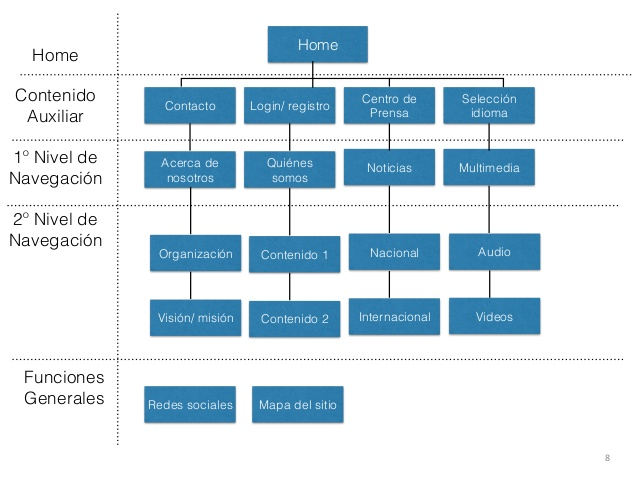
\includegraphics[width=.7\textwidth]{images/mapa}
		\caption{mapa}
		\label{fig:mapa}
	\end{center}
\end{figure}


\cdtInstrucciones{A continuación describa cada una de las pantallas.}
%% !TeX root = ../proyecto.tex
%--------------------------------------
\section{IUX Interfaz (nombre de la interfaz)}

\subsection{Objetivo}
	\cdtInstrucciones{Describa el objetivo, propósito o función de la pantalla.}

\subsection{Diseño}
	\cdtInstrucciones{Describa brevemente los elementos de la pantalla y como de be usarse a manera de manual de usuario.} Esta pantalla \IUref{IU23}{Pantalla de Control de Acceso} aparece al iniciar el sistema, para ingresar ... 

\IUfig[.7]{Login}{IU23}{Pantalla de Control de Acceso.}

%\IUfig[ancho de la figura: valor entre 1 y .1]{Nombre corto de la pantalla sin espacions ni acentos}{IUXX}{Nombre largo de la pantalla.}

\subsection{Salidas}

	\cdtInstrucciones{Liste las salidas de la interfaz. Si coinciden con las del caso de uso solo indiquelo. Esta ,ista debe incluir los mensajes}

	\begin{itemize}
		\item Descripción de salida.
	\end{itemize}
	
\subsection{Entradas}

	\cdtInstrucciones{Liste las entradas de la interfaz. Si coinciden con las del caso de uso solo indiquelo.}
	\begin{itemize}
		\item Descripción de salida.
	\end{itemize}

\subsection{Comandos}
	\cdtInstrucciones{Describa cada control (botónes, areas de drag and drop, componentes interactivos, animaciones, etc.) que se puede utilizar dentro de la pantalla indicando o que hacen y si cambia de pantalla.}

\begin{itemize}
	\item \IUbutton{Entrar}: Verifica que el Estudiante se encuentre registrado y la contraseña sea la correcta. Si la verificación es correcta, se muestra la \IUref{UI32}{Pantalla de Selección de Seminario}.
	\item \IUbutton{Ayuda}: Muestra la ayuda de esta pantalla \IUref{IU50}{Pantalla de Ayuda}.
\end{itemize}


% !TeX root = ../proyecto.tex
%--------------------------------------
\section{IU1 Registrar Cliente}

\subsection{Objetivo}
	\cdtInstrucciones  El objetivo de esta pantalla es permitir al cliente capturar sus datos personales, registrarse en el sistema y poder acceder a las operaciones del sistema definidas para su perfil .


\subsection{Diseño}
	\cdtInstrucciones Esta pantalla \IUref{IU1}{Registrar Cliente} aparece cuando el cliente solicite registarse, para ingresar sus datos personales basta con llenar la informacion desde teclado o mouse, una vez llenados todos los datos podemos hacer click en el boton \IUbutton{Registrar} . 

\IUfig[.7]{RegistroCliente}{IU1}{Registrar Cliente.}

%\IUfig[ancho de la figura: valor entre 1 y .1]{Nombre corto de la pantalla sin espacions ni acentos}{IUXX}{Nombre largo de la pantalla.}

\subsection{Salidas}

	

	\begin{itemize}
		\item Las salidas son las mismas que las del caso de uso \hyperlink{CU1}{CU1 Registrar Cliente}.
	\end{itemize}
	
\subsection{Entradas}

	\cdtInstrucciones{Liste las entradas de la interfaz. Si coinciden con las del caso de uso solo indiquelo.}
	\begin{itemize}
		\item Las entradas son las mismas que las del caso de uso \hyperlink{CU1}{CU1 Registrar Cliente}.
	\end{itemize}

\subsection{Comandos}
	\cdtInstrucciones{Describa cada control (botónes, areas de drag and drop, componentes interactivos, animaciones, etc.) que se puede utilizar dentro de la pantalla indicando o que hacen y si cambia de pantalla.}

\begin{itemize}
	\item \IUbutton{Registrar}: Verifica que los datos personales hayan sido llenados correctamente. Si la verificación es correcta, se muestra la \IUref{UI5}{Pantalla de Home Cliente sin reservaciones}.
	\item \IUbutton{Iniciar sesion}: Muestra la patalla \IUref{IU1.2}{Iniciar sesion}.
\end{itemize}


% !TeX root = ../proyecto.tex
%--------------------------------------
\section{IU2 Pantalla de Datos Obligatorios de la Mascota }

\subsection{Objetivo}
	\cdtInstrucciones El objetivo de esta pantalla es permitir al usuario capturar los datos que son obligatorios de su mascota.

\subsection{Diseño}
	\cdtInstrucciones Esta pantalla \IUref{IU2}{Registrar Mascota} aparece al momento de querer hacer una reservacion, para ingresar los datos de la mascota basta con llenar la informacion desde teclado o mouse, una vez llenados todos los datos podemos hacer click en el boton \IUbutton{Registrar}   

\IUfig[.7]{registrarMascota}{IU2}{Registrar Mascota}

%\IUfig[ancho de la figura: valor entre 1 y .1]{Nombre corto de la pantalla sin espacions ni acentos}{IUXX}{Nombre largo de la pantalla.}

\subsection{Salidas}

	\begin{itemize}
		\item Si los datos de esta pantalla no son llenados, al momento de dar click en el boton \IUbutton{Siguiente}, saltara el mensaje \MSGref{MSG-001}{Campo obligatorio}.
	\end{itemize}
	
\subsection{Entradas}
	\begin{itemize}
		\item Las entradas son las del caso de uso \hyperlink{CU3}{CU3 Registrar Mascota}.
		\item Nombre de la Mascota
		\item Tamaño
		\item Fecha de nacimiento
		\item Especie
		\item Raza
		\item Color de la Mascota
		\item RUAC
		\item Vacunas
	\end{itemize}

\subsection{Comandos}
	%\cdtInstrucciones{Describa cada control (botónes, areas de drag and drop, componentes interactivos, animaciones, etc.) que se puede utilizar dentro de la pantalla indicando o que hacen y si cambia de pantalla.}

\begin{itemize}
	\item \IUbutton{Siguiente}: Verifica que los datos hayan sido llenados. Si la verificación es correcta, se muestra la \IUref{UI3}{Pantalla de Datos Extra de la Mascota}.
\end{itemize}


% !TeX root = ../proyecto.tex
%--------------------------------------
\section{IU2 Pantalla de Datos Obligatorios de la Mascota }

\subsection{Objetivo}
	\cdtInstrucciones El objetivo de esta pantalla es permitir al usuario capturar los datos que son obligatorios de su mascota.

\subsection{Diseño}
	\cdtInstrucciones Esta pantalla \IUref{IU3}{Registrar Mascota} aparece al momento de querer hacer una reservacion, para ingresar los datos de la mascota basta con llenar la informacion desde teclado o mouse, una vez llenados todos los datos podemos hacer click en el boton \IUbutton{Registrar}   

\IUfig[.7]{RegistrarDatosMascota}{IU3}{Registrar Datos Mascota}

%\IUfig[ancho de la figura: valor entre 1 y .1]{Nombre corto de la pantalla sin espacions ni acentos}{IUXX}{Nombre largo de la pantalla.}

\subsection{Salidas}

	\begin{itemize}
		\item Si los datos de esta pantalla no son llenados, al momento de dar click en el boton \IUbutton{Siguiente}, saltara el mensaje \MSGref{MSG-001}{Campo obligatorio}.
	\end{itemize}
	
\subsection{Entradas}
	\begin{itemize}
		\item Las entradas son las del caso de uso \hyperlink{CU3}{CU3 Registrar Mascota}.
		\item Nombre de la Mascota
		\item Tamaño
		\item Fecha de nacimiento
		\item Especie
		\item Raza
		\item Color de la Mascota
		\item RUAC
		\item Vacunas
	\end{itemize}

\subsection{Comandos}
	%\cdtInstrucciones{Describa cada control (botónes, areas de drag and drop, componentes interactivos, animaciones, etc.) que se puede utilizar dentro de la pantalla indicando o que hacen y si cambia de pantalla.}

\begin{itemize}
	\item \IUbutton{Siguiente}: Verifica que los datos hayan sido llenados. Si la verificación es correcta, se muestra la \IUref{UI3}{Pantalla de Datos Extra de la Mascota}.
\end{itemize}


% !TeX root = ../proyecto.tex
%--------------------------------------
\section{IUX Interfaz (nombre de la interfaz)}

\subsection{Objetivo}
	\cdtInstrucciones{Describa el objetivo, propósito o función de la pantalla.}

\subsection{Diseño}
	\cdtInstrucciones{Describa brevemente los elementos de la pantalla y como de be usarse a manera de manual de usuario.} Esta pantalla \IUref{IU23}{Pantalla de Control de Acceso} aparece al iniciar el sistema, para ingresar ... 

\IUfig[.7]{mainPage}{IU3}{Pantalla de inicio.}

%\IUfig[ancho de la figura: valor entre 1 y .1]{Nombre corto de la pantalla sin espacions ni acentos}{IUXX}{Nombre largo de la pantalla.}

\subsection{Salidas}

	\cdtInstrucciones{Liste las salidas de la interfaz. Si coinciden con las del caso de uso solo indiquelo. Esta ,ista debe incluir los mensajes}

	\begin{itemize}
		\item Descripción de salida.
	\end{itemize}
	
\subsection{Entradas}

	\cdtInstrucciones{Liste las entradas de la interfaz. Si coinciden con las del caso de uso solo indiquelo.}
	\begin{itemize}
		\item Descripción de salida.
	\end{itemize}

\subsection{Comandos}
	\cdtInstrucciones{Describa cada control (botónes, areas de drag and drop, componentes interactivos, animaciones, etc.) que se puede utilizar dentro de la pantalla indicando o que hacen y si cambia de pantalla.}

\begin{itemize}
	\item \IUbutton{Entrar}: Verifica que el Estudiante se encuentre registrado y la contraseña sea la correcta. Si la verificación es correcta, se muestra la \IUref{UI32}{Pantalla de Selección de Seminario}.
	\item \IUbutton{Ayuda}: Muestra la ayuda de esta pantalla \IUref{IU50}{Pantalla de Ayuda}.
\end{itemize}


% !TeX root = ../proyecto.tex
%--------------------------------------
\section{IU5 Pantalla Home Cliente}

\subsection{Objetivo}
	\cdtInstrucciones El objetivo de esta pantalla es permitir al cliente ver sus reservacionses, para que de esta forma tenga la opcion de editarlas o eliminarlas, y tambien que tenga la opcion de hacer una reservacion .

\subsection{Diseño}
	\cdtInstrucciones Esta pantalla {UI5}{Pantalla Home Cliente} aparece al momento de registrarse o iniciar sesion, una vez dentro tenemos la opcion de hacer una reservacion dando click en el boton \IUbutton{Reservar}, asi como visualizar nuestras reservaciones y tener la opcion de editar o eliminar la reservacion con los botones \IUbutton{Editar},\IUbutton{Eliminar}.

\IUfig[.7]{Reservaciones}{IU5}{Pantalla de Home Cliente}
\IUfig[.7]{sinReservaciones}{IU5}{Pantalla de Home Cliente sin reservaciones}

%\IUfig[ancho de la figura: valor entre 1 y .1]{Nombre corto de la pantalla sin espacions ni acentos}{IUXX}{Nombre largo de la pantalla.}

\subsection{Salidas}

	%\cdtInstrucciones{Liste las salidas de la interfaz. Si coinciden con las del caso de uso solo indiquelo. Esta ,ista debe incluir los mensajes}

	\begin{itemize}
		\item Si no se ha echo ninguna reservacion, se mostrara el mensaje \MSGref{MSG-003}{No hay reservaciones todavia}.
	\end{itemize}
	
\subsection{Entradas}

	%\cdtInstrucciones{Liste las entradas de la interfaz. Si coinciden con las del caso de uso solo indiquelo.}
	\begin{itemize}
		\item Ninguna
	\end{itemize}

\subsection{Comandos}
	%\cdtInstrucciones{Describa cada control (botónes, areas de drag and drop, componentes interactivos, animaciones, etc.) que se puede utilizar dentro de la pantalla indicando o que hacen y si cambia de pantalla.}

\begin{itemize}
	\item \IUbutton{Hacer reservacion}: Muestra la pantalla \IUref{UI2}{Pantalla de Datos Obligatorios de la Mascota}.
	\item \IUbutton{Editar}: Muestra la pantalla \IUref{UI2}{Pantalla de Datos Obligatorios de la Mascota}, con los datos de esa reservacion y permite modificarlos.
	\item \IUbutton{Eliminar}: Elimina la reservación.
\end{itemize}


% !TeX root = ../proyecto.tex
%--------------------------------------
\section{IU6 Interfaz búsqueda de hospedajes}

\subsection{Objetivo}
	\cdtInstrucciones{Describa el objetivo, propósito o función de la pantalla.}

\subsection{Diseño}
	\cdtInstrucciones{Describa brevemente los elementos de la pantalla y como de be usarse a manera de manual de usuario.} Esta pantalla \IUref{IU23}{Pantalla de Control de Acceso} aparece al iniciar el sistema, para ingresar ... 

\IUfig[0.8]{PANTALLA_BUSQUEDA_HOSPEDAJES}{IU6}{Búsqueda de hospedajes.}

\subsection{Salidas}

	\cdtInstrucciones{Liste las salidas de la interfaz. Si coinciden con las del caso de uso solo indiquelo. Esta ,ista debe incluir los mensajes}

	\begin{itemize}
		\item Descripción de salida.
	\end{itemize}
	
\subsection{Entradas}

	\cdtInstrucciones{Liste las entradas de la interfaz. Si coinciden con las del caso de uso solo indiquelo.}
	\begin{itemize}
		\item Descripción de salida.
	\end{itemize}

\subsection{Comandos}
	\cdtInstrucciones{Describa cada control (botónes, areas de drag and drop, componentes interactivos, animaciones, etc.) que se puede utilizar dentro de la pantalla indicando o que hacen y si cambia de pantalla.}

\begin{itemize}
	\item \IUbutton{Entrar}: Verifica que el Estudiante se encuentre registrado y la contraseña sea la correcta. Si la verificación es correcta, se muestra la \IUref{UI32}{Pantalla de Selección de Seminario}.
	\item \IUbutton{Ayuda}: Muestra la ayuda de esta pantalla \IUref{IU50}{Pantalla de Ayuda}.
\end{itemize}


% !TeX root = ../proyecto.tex
%--------------------------------------
\section{IU7 Interfaz catálogo de habitaciones}

\subsection{Objetivo}
	\cdtInstrucciones{Describa el objetivo, propósito o función de la pantalla.}

\subsection{Diseño}
	\cdtInstrucciones{Describa brevemente los elementos de la pantalla y como de be usarse a manera de manual de usuario.} Esta pantalla \IUref{IU23}{Pantalla de Control de Acceso} aparece al iniciar el sistema, para ingresar ... 

\IUfig[.8]{PANTALLA_CATALOGO_HABITACIONES}{IU7}{Pantalla de catálogo de habitaciones.}

%\IUfig[ancho de la figura: valor entre 1 y .1]{Nombre corto de la pantalla sin espacions ni acentos}{IUXX}{Nombre largo de la pantalla.}

\subsection{Salidas}

	\cdtInstrucciones{Liste las salidas de la interfaz. Si coinciden con las del caso de uso solo indiquelo. Esta lista debe incluir los mensajes}

	\begin{itemize}
		\item Descripción de salida.
	\end{itemize}
	
\subsection{Entradas}

	\cdtInstrucciones{Liste las entradas de la interfaz. Si coinciden con las del caso de uso solo indiquelo.}
	\begin{itemize}
		\item Descripción de salida.
	\end{itemize}

\subsection{Comandos}
	\cdtInstrucciones{Describa cada control (botónes, areas de drag and drop, componentes interactivos, animaciones, etc.) que se puede utilizar dentro de la pantalla indicando o que hacen y si cambia de pantalla.}

\begin{itemize}
	\item \IUbutton{Entrar}: Verifica que el Estudiante se encuentre registrado y la contraseña sea la correcta. Si la verificación es correcta, se muestra la \IUref{UI32}{Pantalla de Selección de Seminario}.
	\item \IUbutton{Ayuda}: Muestra la ayuda de esta pantalla \IUref{IU50}{Pantalla de Ayuda}.
\end{itemize}
% !TeX root = ../proyecto.tex
%--------------------------------------
\section{IU8 Interfaz vista general del cuarto}

\subsection{Objetivo}
	\cdtInstrucciones{Describa el objetivo, propósito o función de la pantalla.}

\subsection{Diseño}
	\cdtInstrucciones{Describa brevemente los elementos de la pantalla y como de be usarse a manera de manual de usuario.} Esta pantalla \IUref{IU23}{Pantalla de Control de Acceso} aparece al iniciar el sistema, para ingresar ... 

\IUfig[.8]{PANTALLA_VISTA_GENERAL}{IU8}{Pantalla de vista general del cuarto.}

%\IUfig[ancho de la figura: valor entre 1 y .1]{Nombre corto de la pantalla sin espacions ni acentos}{IUXX}{Nombre largo de la pantalla.}

\subsection{Salidas}

	\cdtInstrucciones{Liste las salidas de la interfaz. Si coinciden con las del caso de uso solo indiquelo. Esta ,ista debe incluir los mensajes}

	\begin{itemize}
		\item Descripción de salida.
	\end{itemize}
	
\subsection{Entradas}

	\cdtInstrucciones{Liste las entradas de la interfaz. Si coinciden con las del caso de uso solo indiquelo.}
	\begin{itemize}
		\item Descripción de salida.
	\end{itemize}

\subsection{Comandos}
	\cdtInstrucciones{Describa cada control (botónes, areas de drag and drop, componentes interactivos, animaciones, etc.) que se puede utilizar dentro de la pantalla indicando o que hacen y si cambia de pantalla.}

\begin{itemize}
	\item \IUbutton{Entrar}: Verifica que el Estudiante se encuentre registrado y la contraseña sea la correcta. Si la verificación es correcta, se muestra la \IUref{UI32}{Pantalla de Selección de Seminario}.
	\item \IUbutton{Ayuda}: Muestra la ayuda de esta pantalla \IUref{IU50}{Pantalla de Ayuda}.
\end{itemize}


% !TeX root = ../proyecto.tex
%--------------------------------------
\section{IU9 Interfaz servicios adicionales}

\subsection{Objetivo}
	\cdtInstrucciones{Describa el objetivo, propósito o función de la pantalla.}

\subsection{Diseño}
	\cdtInstrucciones{Describa brevemente los elementos de la pantalla y como de be usarse a manera de manual de usuario.} Esta pantalla \IUref{IU23}{Pantalla de Control de Acceso} aparece al iniciar el sistema, para ingresar ... 

\IUfig[.7]{PANTALLA_SERVICIOS_EXTRA}{IU9}{Pantalla de servicios adicionales.}

%\IUfig[ancho de la figura: valor entre 1 y .1]{Nombre corto de la pantalla sin espacions ni acentos}{IUXX}{Nombre largo de la pantalla.}

\subsection{Salidas}

	\cdtInstrucciones{Liste las salidas de la interfaz. Si coinciden con las del caso de uso solo indiquelo. Esta ,ista debe incluir los mensajes}

	\begin{itemize}
		\item Descripción de salida.
	\end{itemize}
	
\subsection{Entradas}

	\cdtInstrucciones{Liste las entradas de la interfaz. Si coinciden con las del caso de uso solo indiquelo.}
	\begin{itemize}
		\item Descripción de salida.
	\end{itemize}

\subsection{Comandos}
	\cdtInstrucciones{Describa cada control (botónes, areas de drag and drop, componentes interactivos, animaciones, etc.) que se puede utilizar dentro de la pantalla indicando o que hacen y si cambia de pantalla.}

\begin{itemize}
	\item \IUbutton{Entrar}: Verifica que el Estudiante se encuentre registrado y la contraseña sea la correcta. Si la verificación es correcta, se muestra la \IUref{UI32}{Pantalla de Selección de Seminario}.
	\item \IUbutton{Ayuda}: Muestra la ayuda de esta pantalla \IUref{IU50}{Pantalla de Ayuda}.
\end{itemize}


% !TeX root = ../proyecto.tex
%--------------------------------------
\section{IU10 Interfaz registrar más detalles}

\subsection{Objetivo}
	\cdtInstrucciones{Describa el objetivo, propósito o función de la pantalla.}

\subsection{Diseño}
	\cdtInstrucciones{Describa brevemente los elementos de la pantalla y como de be usarse a manera de manual de usuario.} Esta pantalla \IUref{IU23}{Pantalla de Control de Acceso} aparece al iniciar el sistema, para ingresar ... 

\IUfig[.8]{PANTALLA_REGISTRAR_MAS_DETALLES}{IU10}{Pantalla de registrar más detalles.}

%\IUfig[ancho de la figura: valor entre 1 y .1]{Nombre corto de la pantalla sin espacions ni acentos}{IUXX}{Nombre largo de la pantalla.}

\subsection{Salidas}

	\cdtInstrucciones{Liste las salidas de la interfaz. Si coinciden con las del caso de uso solo indiquelo. Esta ,ista debe incluir los mensajes}

	\begin{itemize}
		\item Descripción de salida.
	\end{itemize}
	
\subsection{Entradas}

	\cdtInstrucciones{Liste las entradas de la interfaz. Si coinciden con las del caso de uso solo indiquelo.}
	\begin{itemize}
		\item Descripción de salida.
	\end{itemize}

\subsection{Comandos}
	\cdtInstrucciones{Describa cada control (botónes, areas de drag and drop, componentes interactivos, animaciones, etc.) que se puede utilizar dentro de la pantalla indicando o que hacen y si cambia de pantalla.}

\begin{itemize}
	\item \IUbutton{Entrar}: Verifica que el Estudiante se encuentre registrado y la contraseña sea la correcta. Si la verificación es correcta, se muestra la \IUref{UI32}{Pantalla de Selección de Seminario}.
	\item \IUbutton{Ayuda}: Muestra la ayuda de esta pantalla \IUref{IU50}{Pantalla de Ayuda}.
\end{itemize}


% !TeX root = ../proyecto.tex
%--------------------------------------
\section{IU11 Interfaz resumen del hospedaje}

\subsection{Objetivo}
	\cdtInstrucciones{Describa el objetivo, propósito o función de la pantalla.}

\subsection{Diseño}
	\cdtInstrucciones{Describa brevemente los elementos de la pantalla y como de be usarse a manera de manual de usuario.} Esta pantalla \IUref{IU23}{Pantalla de Control de Acceso} aparece al iniciar el sistema, para ingresar ... 

\IUfig[.7]{RESUMEN_HOSPEDAJE}{IU11}{Pantalla de resumen del hospedaje.}

%\IUfig[ancho de la figura: valor entre 1 y .1]{Nombre corto de la pantalla sin espacions ni acentos}{IUXX}{Nombre largo de la pantalla.}

\subsection{Salidas}

	\cdtInstrucciones{Liste las salidas de la interfaz. Si coinciden con las del caso de uso solo indiquelo. Esta ,ista debe incluir los mensajes}

	\begin{itemize}
		\item Descripción de salida.
	\end{itemize}
	
\subsection{Entradas}

	\cdtInstrucciones{Liste las entradas de la interfaz. Si coinciden con las del caso de uso solo indiquelo.}
	\begin{itemize}
		\item Descripción de salida.
	\end{itemize}

\subsection{Comandos}
	\cdtInstrucciones{Describa cada control (botónes, areas de drag and drop, componentes interactivos, animaciones, etc.) que se puede utilizar dentro de la pantalla indicando o que hacen y si cambia de pantalla.}

\begin{itemize}
	\item \IUbutton{Entrar}: Verifica que el Estudiante se encuentre registrado y la contraseña sea la correcta. Si la verificación es correcta, se muestra la \IUref{UI32}{Pantalla de Selección de Seminario}.
	\item \IUbutton{Ayuda}: Muestra la ayuda de esta pantalla \IUref{IU50}{Pantalla de Ayuda}.
\end{itemize}




%!TEX root = ejemplo.tex
%=========================================================
\section{Catálogo de mensajes}	
\label{sec:mensajes}

	En esta sección se describen todos los mensajes que aparecen en el sistema. Para cada mensaje se especifica:
	 
	\begin{description}\itemsep0em
		\item[Id:] Identificador del mensaje de la forma ``MSG XX'' y descripción corta del mismo.
		\item[Tipo:] Tipo del mensaje el cual puede ser: 
		\begin{description}
			\item[Normal:] Mensaje que informa al usuario una instrucción o el estado interno que guarda el sistema, suele tener un color {\color{msgNormalColor}Azul}.
			\item[Éxito:] Mensaje que informa al usuario sobre una acción realizada, sirve para confirmar el correcto funcionamiento del sistema. Se presentan con un color {\color{msgInfoColor}Verde}.
			\item[Atención:] Mensaje que tiene como finalidad llamar la atención del usuario a una situación que requiere su intervención, por ejemplo cuando una actividad ha generado un efecto colateral o se realizará una acción destructiva y no reversible. Se presentan con un color {\color{msgWarningColor}Naranja}.
			\item[Error:] Mensaje que informa al usuario un fallo en en una operación o un impedimento para realizarla, por ejemplo: cuando no se puede efectuar la acción solicitada, cuando un dato falta o tiene un formato no aceptado por el sistema. Se presentan con un color {\color{msgErrorColor}Rojo}.
		\end{description}
		\item[Propósito:] Explicación del propósito del mensaje.
		\item[Redacción:] Redacción del mensaje.
		\item[Parámetros:] En caso de que el mensaje pueda variar se especifican los casos y la forma en que debe adaptarse la redacción
		\item[Ejemplos:] Ejemplos de como debe renderizarse el mensaje.
	\end{description}


\subsection{Lista de mensajes}
%msgNormalColor
%msgInfoColor
%msgWarninigColor
%msgErrorColor

%Mensaje establecido y en uso
\begin{cdtMessage}[msgErrorColor]{MSG-001}{Campo obligatorio}
	\item[Propósito:] Indicar al usuario que existen campos vacíos en su petición que son obligatorios para completar con éxito la operación
	\item[Redacción:] El campo "$<$atributo$>$" debe ser llenado para continuar.
	\item[Parámetros:] \hspace{1cm}
	\begin{itemize}
		\item $<$atributo$>$ se refiere al nombre del atributo que se está dejando vacío en la petición.
	\end{itemize}
	\item[Ejemplos:] El campo $"$CURP$"$ debe ser llenado para continuar.
\end{cdtMessage}

%Mensaje sin establecer ni usar
\begin{cdtMessage}[msgErrorColor]{MSG-002}{RUAC ya existente} 
	\item[Propósito:] Indicar al usuario que el RUAC ingresado para la mascota ya se encuentra asociado a otra en el sistema.
	\item[Redacción:] El RUAC $<$RUAC$>$ ya se encuentra asociado a otra mascota.
	\item[Parámetros:] \hspace{1cm}
	\begin{itemize}
		\item $<$RUAC$>$ Se refiere al \hyperlink{mascota.RUAC}{RUAC} que el usuario desea asociar a su mascota.
	\end{itemize}
	\item[Ejemplos:] El RUAC PHCXA50604 ya se encuentra asociado a otra mascota.
\end{cdtMessage}

%Mensaje establecido y en uso
\begin{cdtMessage}[msgErrorColor]{MSG-003}{No hay reservaciones} 
	\item[Propósito:] Indicar al cliente que no tiene reservaciones realizadas o sin pagar.
	\item[Redacción:] No tienes reservaciones. ¿Deseas realizar una?.
	\item[Parámetros:] No aplica.
	\item[Ejemplos:] No tienes reservaciones. ¿Deseas realizar una?.
\end{cdtMessage}

%Mensaje establecido y en uso
\begin{cdtMessage}[msgErrorColor]{MSG-004}{Vacunas obligatorias}
	\item[Propósito:] Indicar al usuario que para poder registrar a su mascota y sea aceptada para hospedarse en el hotel debe contar con las 3 vacunas mínimas obligatorias.
	\item[Redacción:] Por tu seguridad y la de los demás, tu mascota debe contar con las 3 vacunas mínimas obligatotias.
	\item[Parámetros:] No aplica.
	\item[Ejemplos:] Por tu seguridad y la de los demás, tu mascota debe contar con las 3 vacunas mínimas obligatotias.
\end{cdtMessage}

%Mensaje establecido y en uso
\begin{cdtMessage}[msgErrorColor]{MSG-005}{CURP ya existente}
	\item[Propósito:] Indica al usuario que el CURP con el que intenta registrarse ya es ocupado por otro perfil.
	\item[Redacción:] El CURP introducido ya está registrado en otro perfil.
	\item[Parámetros:] No aplica.
	\item[Ejemplos:] El CURP introducido ya está registrado en otro perfil.
\end{cdtMessage}

%Mensaje establecido y en uso
\begin{cdtMessage}[msgErrorColor]{MSG-006}{Correo electrónico ya existente}
	\item[Propósito:] Indicar al usuario que el correo electrónico con el que intenta registrarse ya es ocupado por otro perfil.
	\item[Redacción:] El correo electrónico introducido ya está registrado en otro perfil.
	\item[Parámetros:] No aplica.
	\item[Ejemplos:] El correo electrónico introducido ya está registrado en otro perfil.
\end{cdtMessage}

%Mensaje establecido y en uso
\begin{cdtMessage}[msgErrorColor]{MSG-007}{Dato no válido}
	\item[Propósito:] Indicar al usuario que uno o más campos están siendo llenados con formatos no válidos en su solicitud para poder realizar con éxito la operación.
	\item[Redacción:] Introduzca valores válidos en los campos correspondientes.
	\item[Parámetros:] No aplica.
	\item[Ejemplos:] Introduzca valores válidos en los campos correspondientes.
\end{cdtMessage}

%Mensaje establecido y en uso
\begin{cdtMessage}[msgErrorColor]{MSG-008}{Fecha no disponible} 
	\item[Propósito:] Indicar al usuario que en las fechas que selecciona su hospedaje no hay cuartos disponibles con las características solicitadas.
	\item[Redacción:] Lo sentimos, no hay cuartos disponibles para el periodo del $<$check-in$>$ al $<$check-out$>$ con las características requeridas. Seleccione otro periodo. 
	\item[Parámetros:] \hspace{1cm}
	\begin{itemize}
		\item $<$check-in$>$ Fecha proyectada de llegada y en la que se inicia el periodo de hospedaje.
		\item $<$check-out$>$ Fecha proyectada de salida y en la que se finaliza el periodo de hospedaje.
	\end{itemize}
	\item[Ejemplos:] \hspace{1cm}
	\begin{itemize}
		\item Lo sentimos, no hay cuartos disponibles para el periodo del 07-05-2024 al 09-05-2024 con las características requeridas. Seleccione otro periodo. 
	\end{itemize}
\end{cdtMessage}
